\chapter{Software pro zařízení}

Tato kapitola se věnuje návrhu a vývoji software pro výsledné zařízení včetně zpracování přijatých dat na serveru a jejich zobrazení uživateli v grafické podobě. Jako první jsou rozebrány možnosti zpracovávání dat a na základě výběru vhodných služeb pro tyto účely je navržen obslužný firmware mikrokontroleru a další součásti zpracování dat.

\section{Server pro zpracování naměřených dat}

Důležitým rozhodnutím pro realizaci celého zařízení je vhodný výběr aplikací a služeb, ve kterých se budou naměřená data uchovávat a následně zpracovávat či zobrazovat. Na trhu existuje několik veřejně dostupných serverů, které umožňují přijímání dat skrze různé protokoly a jejich následné uchovávání a zpracovávání.

Mezi nejznámější služby patří ThingSpeak\footnote{\url{https://thingspeak.com/}}, který umožňuje integraci MATLAB skriptů které se spouštějí nad uloženými přijatými daty. Při využívání neplacené verze této služby jsme limitování maximálním počtem přijatých zpráv za den (\SI{8200}{}), maximální dobou běhu skriptů \SI{20}{\second} nebo třeba pouze čtyřmi neveřejnými kanály na jeden účet. Další nevýhodou je možnost přijímat do jednoho kanálu maximálně 8 proměnných, pokud bychom chtěli vizualizovat více dat, musíme je rozdělit do více kanálů a můžeme tak brzy narazit na limity účtu poskytovaného zdarma.

Dalším z možných serverů na příjem a zpracování dat je ubidots\footnote{\url{https://ubidots.com/}}. I tento server poskytuje licenci zdarma, která je určena pro nekomerční použití studenty a kutily, kteří si chtějí platformu vyzkoušet. Nachází se zde omezení například v počtu maximálně tří připojených zařízení a uchovávání dat po dobu maximálně jednoho měsíce. Každé připojené zařízení může zasílat ke zpracování maximálně \SI{10}{} měřených veličin.

Jednou z možností je využít Arduino Cloud\footnote{\url{https://docs.arduino.cc/cloud/iot-cloud}} od stejnojmenné společnosti Arduino. Jejich cloud nabízí také plán pro používání bez poplatků, zde se dostáváme na mnohem větší restrikce než u dříve zmíněných služeb. Připojena mohou být pouze dvě zařízení, zařízení musí být naprogramováno v jejich prostředí, jelikož není k dispozici API pro připojení jiných zařízení. Největší nevýhodou je uchovávání naměřených dat pouze jeden den, což je pro statistiky či sledování nepoužitelné.

Další z mnoha možností, jak uchovávat a zpracovávt naměřená data je vytvoření vlastního prostředí pro tyto účely. Lze použít spojení databázové aplikace, která bude uchovávat data (např. InfluxDB\footnote{\url{https://www.influxdata.com/}}) a dalších služeb pro příjem, zpracování a zobrazení těchto dat. Pro příjem zpráv od zařízení bude připojen Eclipse Mosquitto\footnote{\url{https://mosquitto.org/}}, což je tzv. MQTT broker, který je potřebný k přijímání dat zasílaných skrze protokol MQTT. Tento broker lze poté připojit přes Node-RED\footnote{\url{https://nodered.org/}}, což je programovací nástroj určený k jednoduchému propojení zařízení s dalšími službami, lze jej tedy použít pro zpracování přijatých zpráv a jejich následné uložení do databáze. Statistiky a přehledy lze vykreslovat pomocí služby Grafana\footnote{\url{https://grafana.com/}}. Všechny tyto nástroje jsou open-source a lze je využívat zdarma i pro komerční použití.

\section{Základní funkce zařízení}

Na obrázku \ref{fig_flowchart} je vidět základní koncept běhu programu pro mikrokontroler. Jedná se o jednoduchý stavový automat, který zajistí vykonání příkazů ve správném pořadí a zajišťuje čekání na přijmutí dat ze všech senzorů. V tomto zařízení jsou totiž využity senzory, které neposkytují změřená data okamžitě, ale až po delším časovém úseku svého provozu. Například senzor SGP30 pro měření TVOC a koncentrace CO$_2$ vrací prvních \SI{15}{\second} fixní hodnotu 400~ppm a až po uplynutí tohoto času začne vracet reálná naměřená data. Velice podobně pracuje i senzor koncentrace prachových částic, kde potřebuje být v provozu alespoň \SI{20}{\second} aby dokázal vrátit naměřená data.

\begin{figure}[h]
    \centering
    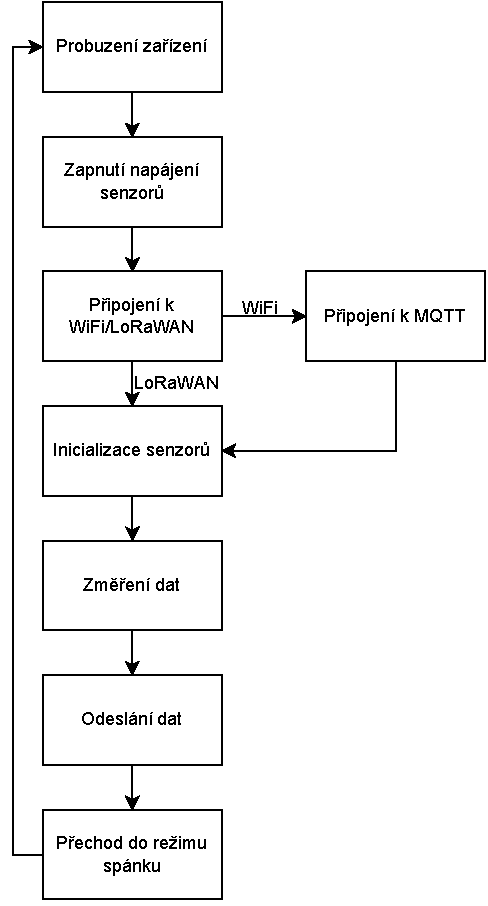
\includegraphics[width=0.4\textwidth]{obrazky/flowchart.pdf}
    \caption{Základní funkce softwaru pro mikrokontroler.}
    \label{fig_flowchart}
\end{figure}

Jak již bylo zmíněno v předchozích kapitolách, zařízení bude moci zasílat naměřená data pomocí WiFi nebo pomocí LoRaWAN sítě. Obě dvě sítě vyžadují projít procesem připojení, kde u WiFi zařízení dostane přidělenou IP adresu a u LoRaWAN dojde k vygenerování klíčů, pomocí kterých se poté šifrují a zasílají zprávy. Zařízení je koncipováno tak, že může být připojeno pouze k jedné z těchto sítí a toto nastavení je definováno pevně ve firmwaru zařízení. 

\section{Firmware mikrokontroleru}

